\section{Project Management}\label{sec:projectmanagement}
According to Section~\ref{subsec:sdp} we are using Software Development Life Cycle (SDLC) as our software development process. There are various method of SDLC. Among them we are using Agile SDLC method. Also, there are various Agile methodologies. Here we are using Scrum methodology. This can be shown as follows.

\begin{figure}[H]
    \centering
    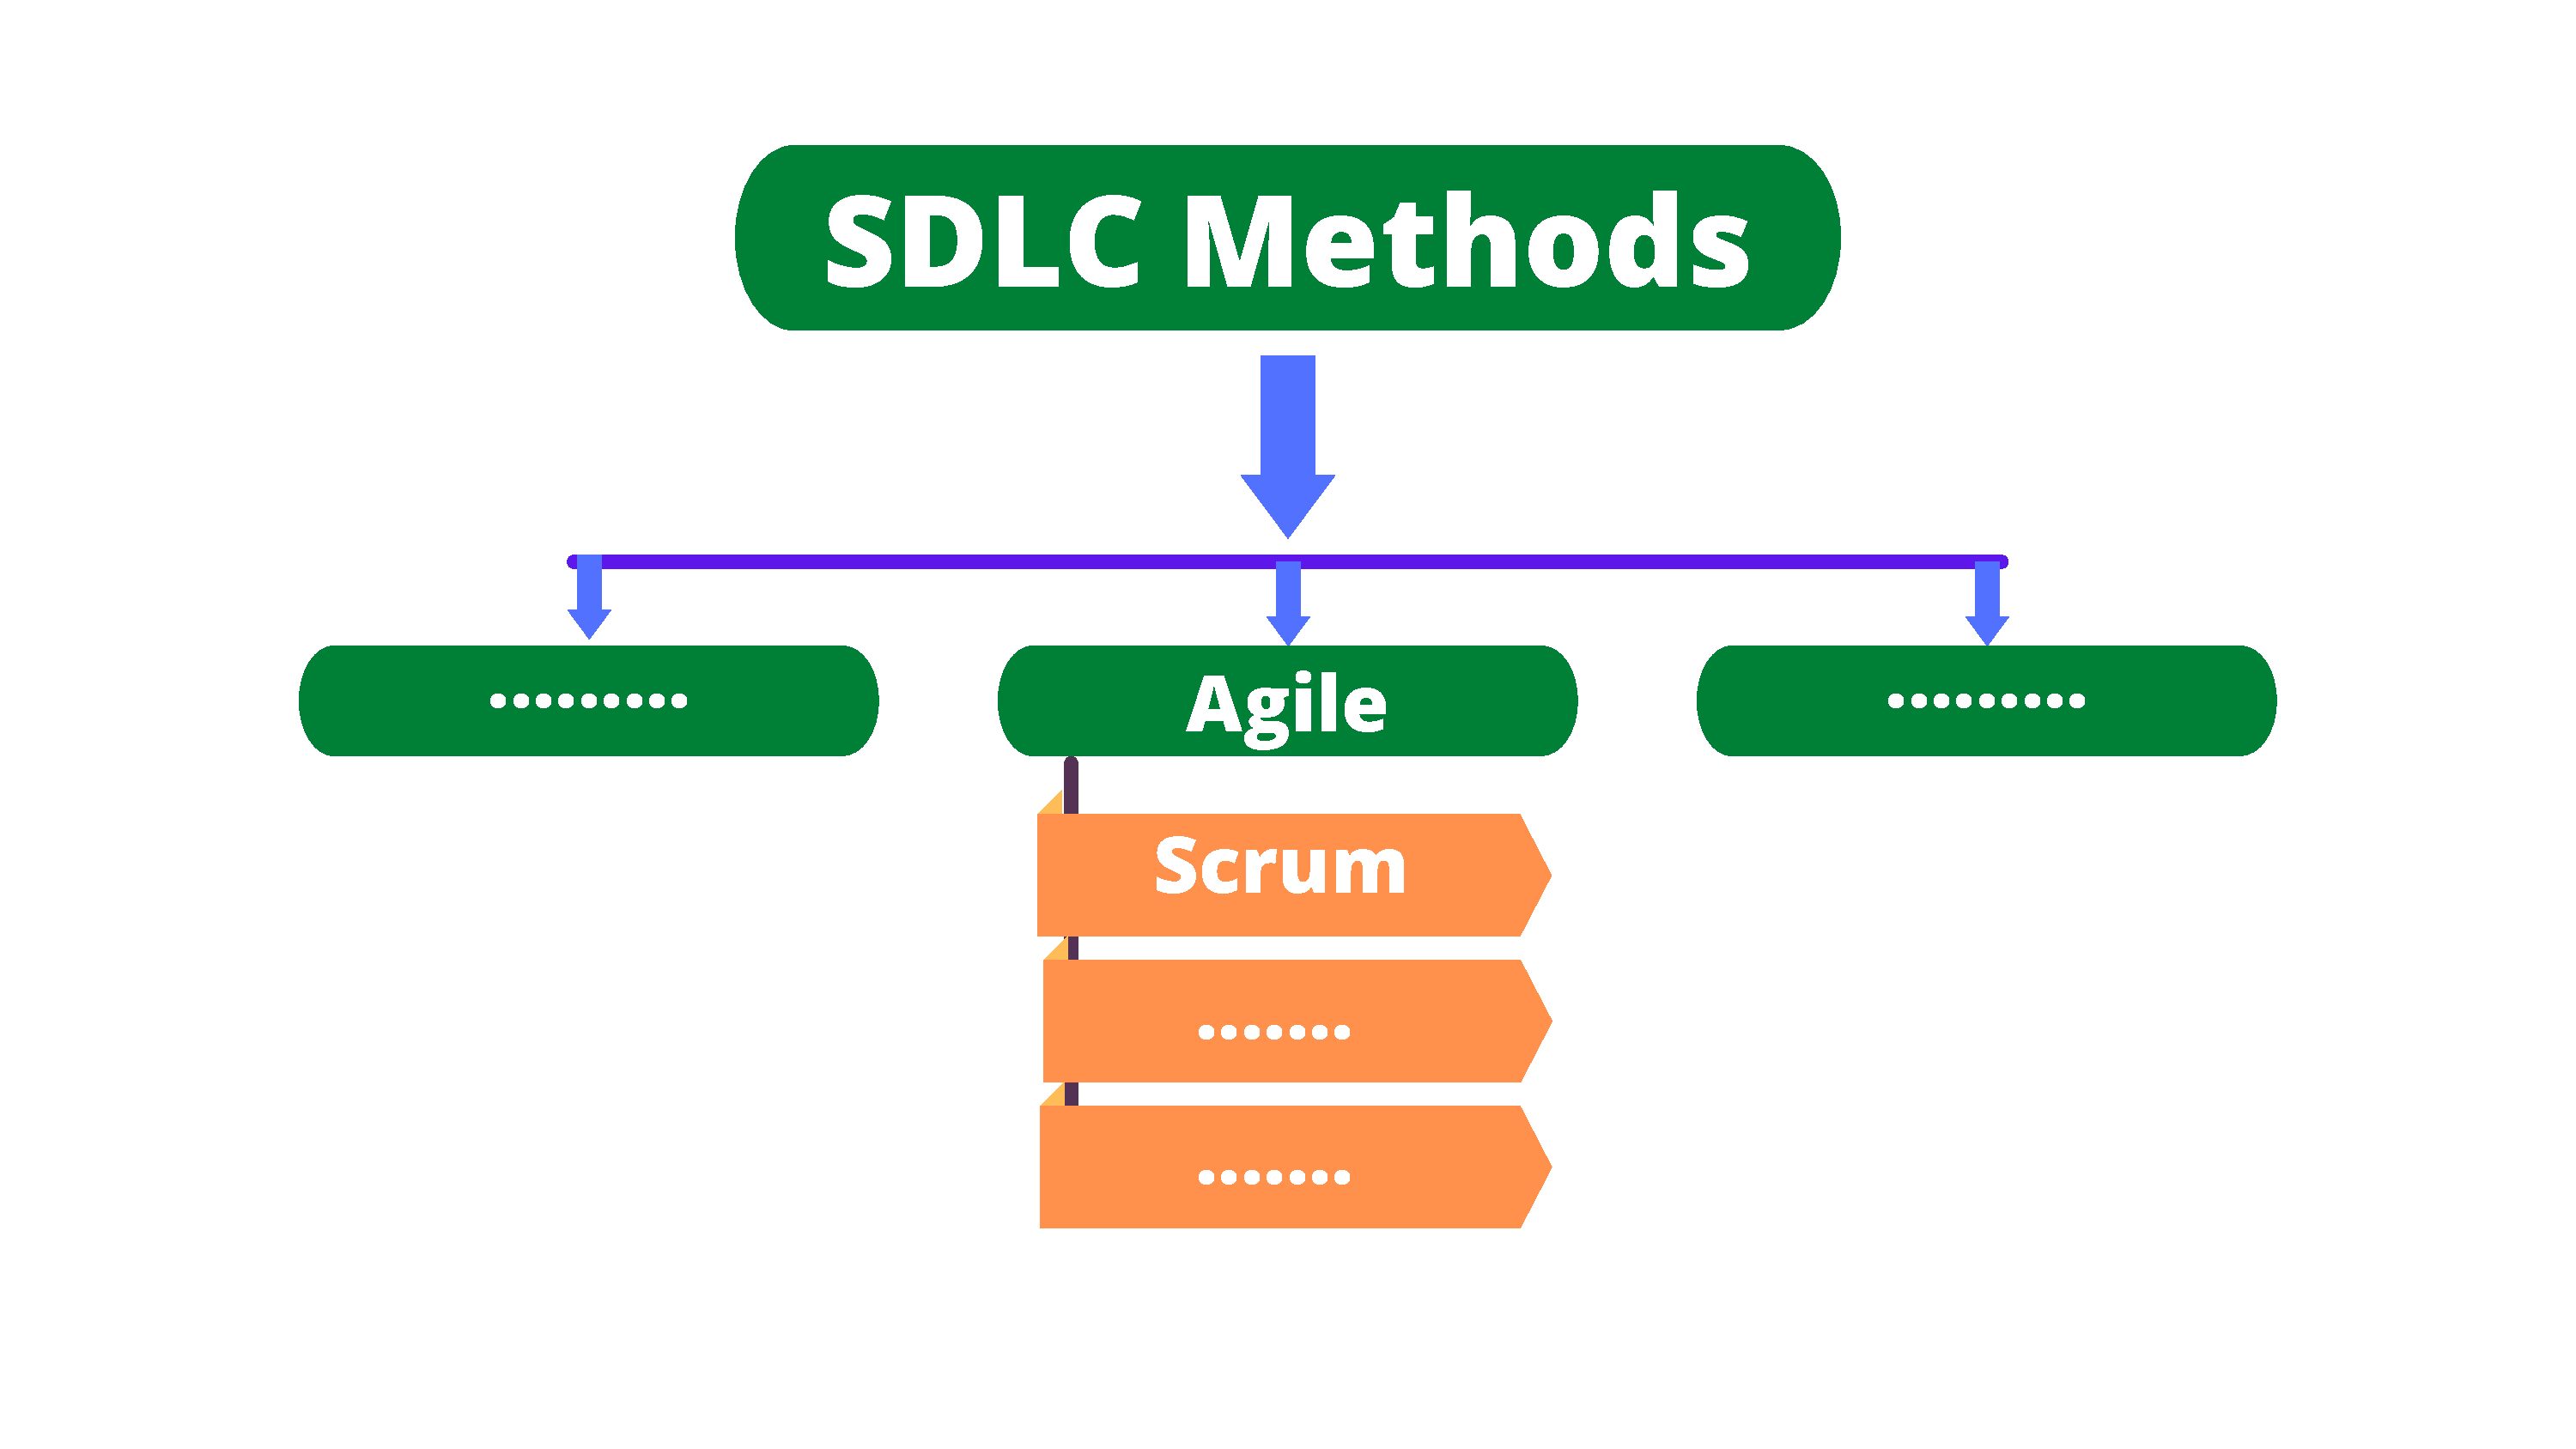
\includegraphics[width=1\textwidth]{images/SDLCMethods}
    \caption{SDLC classification}
    \label{fig:sdlc-class}
\end{figure}

The Agile SDLC model is a combination of iterative and incremental process models with a focus on process adaptability and customer satisfaction by rapid delivery of working software products. Agile Methods break the product into small incremental builds. These builds are provided in iterations. Each iteration typically lasts from about one to three weeks.
Every iteration involves cross-functional teams working simultaneously on various areas like −
\begin{itemize}
\item Planning/Requirement Gathering
\item Requirements Analysis
\item Database Modeling
\item Architectural Design
\item Implementation
\item Testing and Validation
\end{itemize}

Ref: [www.tutorialspoint.com/sdlc/sdlc\_agile\_model.htm]
Agile model believes that every project needs to be handled differently and the existing methods need to be tailored to best suit the project requirements. In Agile, the tasks are divided to time boxes (small time frames) to deliver specific features for a release.\\

Iterative approach is taken and working software build is delivered after each iteration. Each build is incremental in terms of features; the final build holds all the features required by the customer.


Here is a graphical illustration of the Agile Model −
\begin{figure}[H]
    \centering
    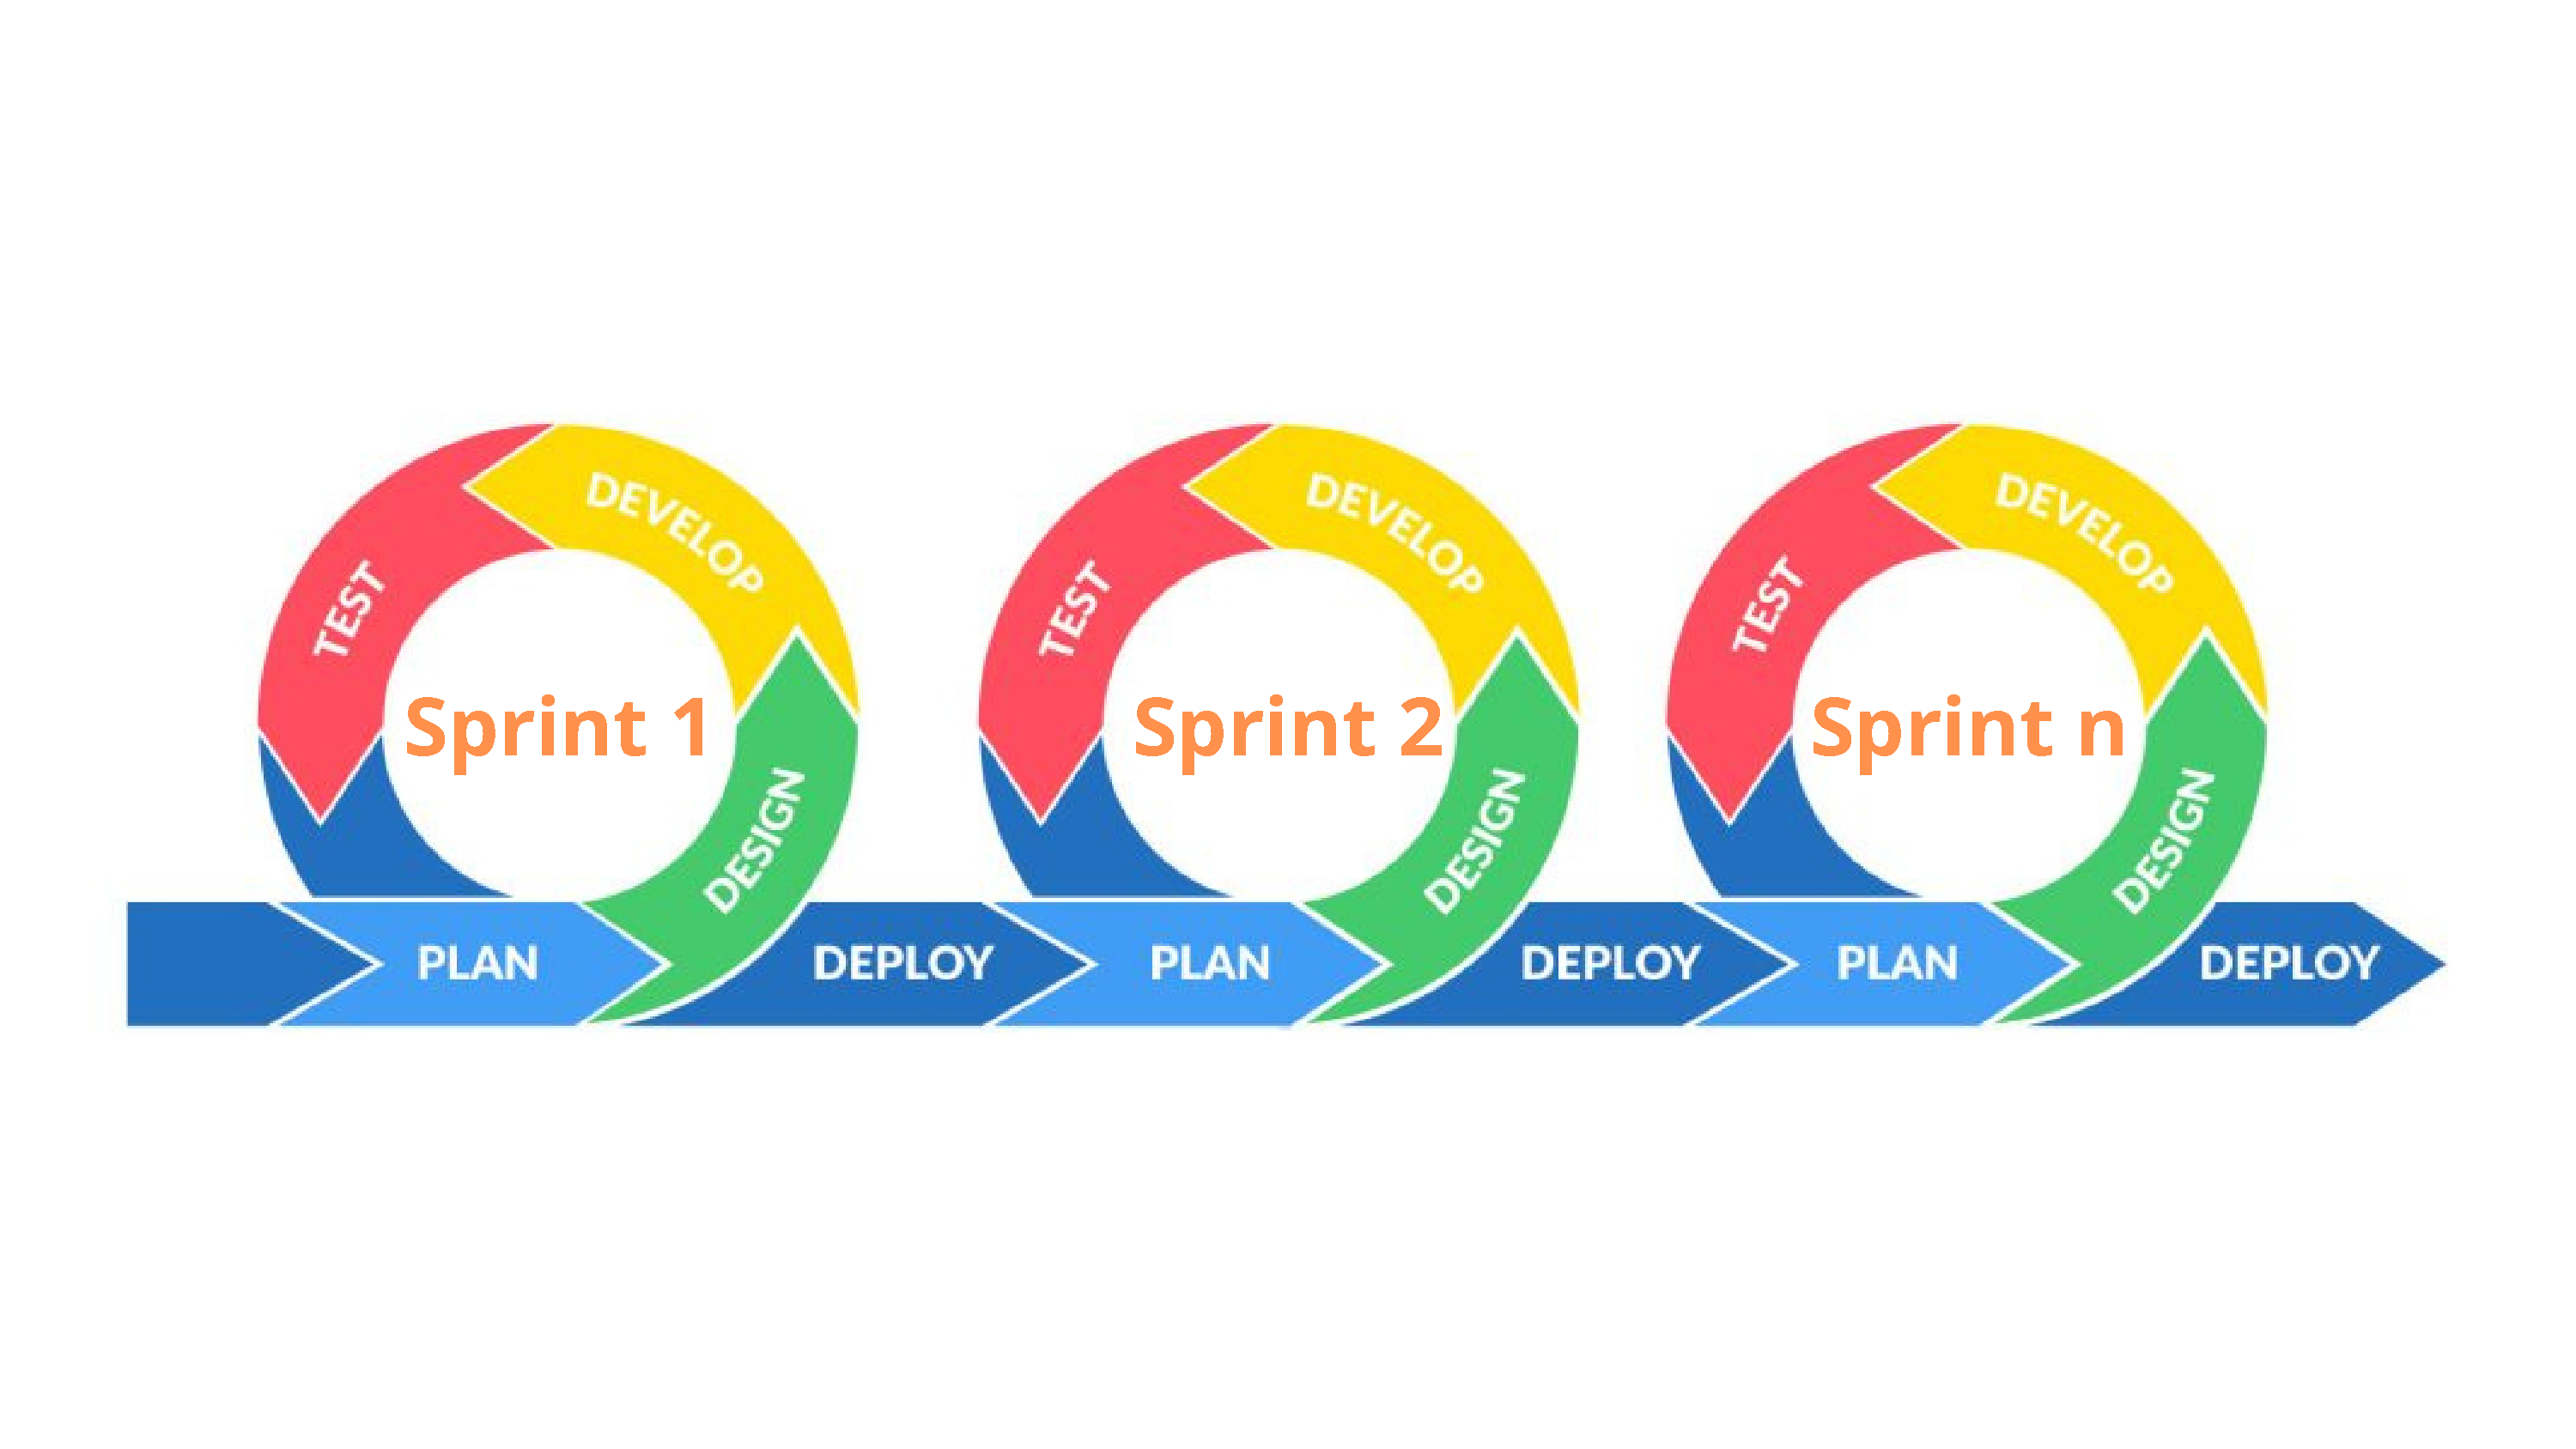
\includegraphics[width=1\textwidth]{images/agile}
    \caption{Agile Model}
    \label{fig:agile}
\end{figure}
We define separate phases (sprints in Scrum terminology) for each and every steps of SDLC. For each phase we make a plan, design a work-flow, develop it, and finally test the output of the phase. If the output is correct according to the requirements, then we proceed for the next phase.\\

To complete each of these phases or sprints we followed the Scrum methodology. It actually allows implementing Agile development methodology. So it can be called a framework which enables an iterative and incremental development process. At the end of each step a usable product is delivered to a customer. Customer feedback helps reveal possible problems or change the initial development plan if needed.\\
Here are the main roles involved in the development process, according to the Scrum model:
\begin{description}
\item[Product owner :] The product owner takes care of the end user’s interests;
\item[Scrum master :] The Scrum master coordinates the whole development process. Another task is to make sure that Scrum is used properly and to hold regular Scrum meetings;
\item[Scrum team :] The Scrum team develops the product. Its main tasks are programming, analysis, testing, etc.
\end{description}
Now, let’s take a look at the main steps of the development process that Scrum consists of which we followed.

\begin{enumerate}
\item \textbf{Product Backlog Creation}\\
In this process, we transformed the significance and functional details of the system into short stories. Every user story gets a unique ID. As a rule, user stories have the following format: As a [User Role], I want to [feature body] so that [User profit]. This list below shows how these stories can look like. These are actual product requirements that were implemented during the software developing process:
\begin{table}[h]
\centering
\huge
\resizebox{\textwidth}{!}{
\begin{tabular}{|l|l|l|}
\hline
UserID & User Type & User Story \\ \hline
user-01 & Student & I want to pay all my tuition fees via online from anywhere in the world. \\ \hline
user-02 & Student & I want to see all of my previous transactions and due transactions that I need to complete. \\ \hline
user-003 & Administrative personnel & I need to create, update and edit payments for each and every students. \\ \hline
user-04 & Administrative personnel & I want to have track of the payments for all the students. \\ \hline
user-05 & Teacher & I need to collect attendance online for each and every classes I take. \\ \hline
\end{tabular}
}
\caption{\label{tab:userStory}User story example.}
\end{table}

After listing all the product backlog items, it's time to sort through them and prioritize the tasks that which tasks are more important than others. Most important one is ranked higher than less important one. This is called prioritization. We then make a list ordering according to the priority in descending order. This one is a continuous process. Because we continuously add a new item in the backlog list and prioritize it and update the listing.



%As an example, consider a standard student whose semester final test is scheduled for a few days from now. He/she will be required to pay the semester fee within a certain time frame determined by the administration. Students suffer as a result of this, and their preparedness is negatively impacted. Furthermore, while using the traditional method of transaction, a university is completely reliant on a single bank branch, which creates a tiring and agonizing scenario when a large number of students seek to pay their tuition fees on the same day as the university. Several students even fail to submit their fees on time since they are unable to conduct any financial activities during non-working hours. Teachers are also said to have lost around one-third of the course session while manually collecting attendance, which has an adverse impact on the focus of pupils. On the other aspect, management often complains about how time-consuming it is to manually update student data in papers. It not only takes a long time to finish, but it also needs the actual presence of a huge number of individuals in order to be successful. These considerations inspired our team's decision to design a single application using the information obtained from our database course that is capable of resolving all of the challenges discussed above.%

\item \textbf{Sprint planning and creating backlog}\\

It was then time for the establishment of the sprint backlog, for which our team had to choose the most essential user stories and split them down into smaller tasks. Contingency plan was developed for how we would execute the work. In addition, our team prioritized the activities that needed to be completed in order to complete the project more efficiently. The sprint lasted around 9 to 10 days, which was sufficient time for the developers to complete their task completely.

\item \textbf{Working on sprint}\\

This was a phase of practical application. The real stories were reorganized as discrete tasks in the sprint backlog, which is where the actual work began. In order to get started, a task board, also known as a Kanban board in Trello\footnotemark , was created with a large number of cards in use. Using the cards, you may describe the specifics of the tasks, such as who will be assigned to the job, what will be done, when it will be completed, and so on. Additionally, we utilized these cards to keep track of our meeting schedule and information, as well as any future revisions. In addition to the ``To Do" lists, the task board also had columns for ``Work In Progress," ``Testing," and ``Work Done," as well as a column for "Testing." A typical task board is shown in the diagram below.
\\

In the scrum approach, a project is often completed by combining the efforts of a large group of people who are all overseen by a single individual. In our situation, \textit{Md Masud Majumdar} was the team's leader from the beginning to the conclusion, and he planned and executed the whole project. Each team member has made significant contributions to various aspects of the overall project.\\

We held regular virtual meetings where all the teammates together, came up with all the various ideas to design the database schema. The meetings we held virtually through Google Meet\footnotemark and Zoom software were led by \textit{Tareq Rahman Khan}. Within a week, we decided to draw the first E-R Diagram on our ideas which was fianlly done by \textit{Palash Hossen}. Later it was modified by \textit{Nu Sai Mong Marma}.\\

While developing the system, we used Github\footnotemark to make the collaboration among teammates and to integrate all the assigned task and make the final system. Github not only allowed us to collaborate with our teammates but also to control the modifications of the application. Since the start of the project, our team made about 100 of commits into Github repository. All the commits are from \textit{Tonmoy Chandro Das} and \textit{Md. Masud Majumdar} as frontend and backend funcionalities were developed by them. To interact with github, we used git in our local machine and Visual Studio Code as code editor.\\

While developing the system, we also looked after the documentation of this entire project. This documentation was prepared under the leadership of \textit{Hamza Mohtadee Nafi}.\\

\begin{figure}[H]
    \centering
    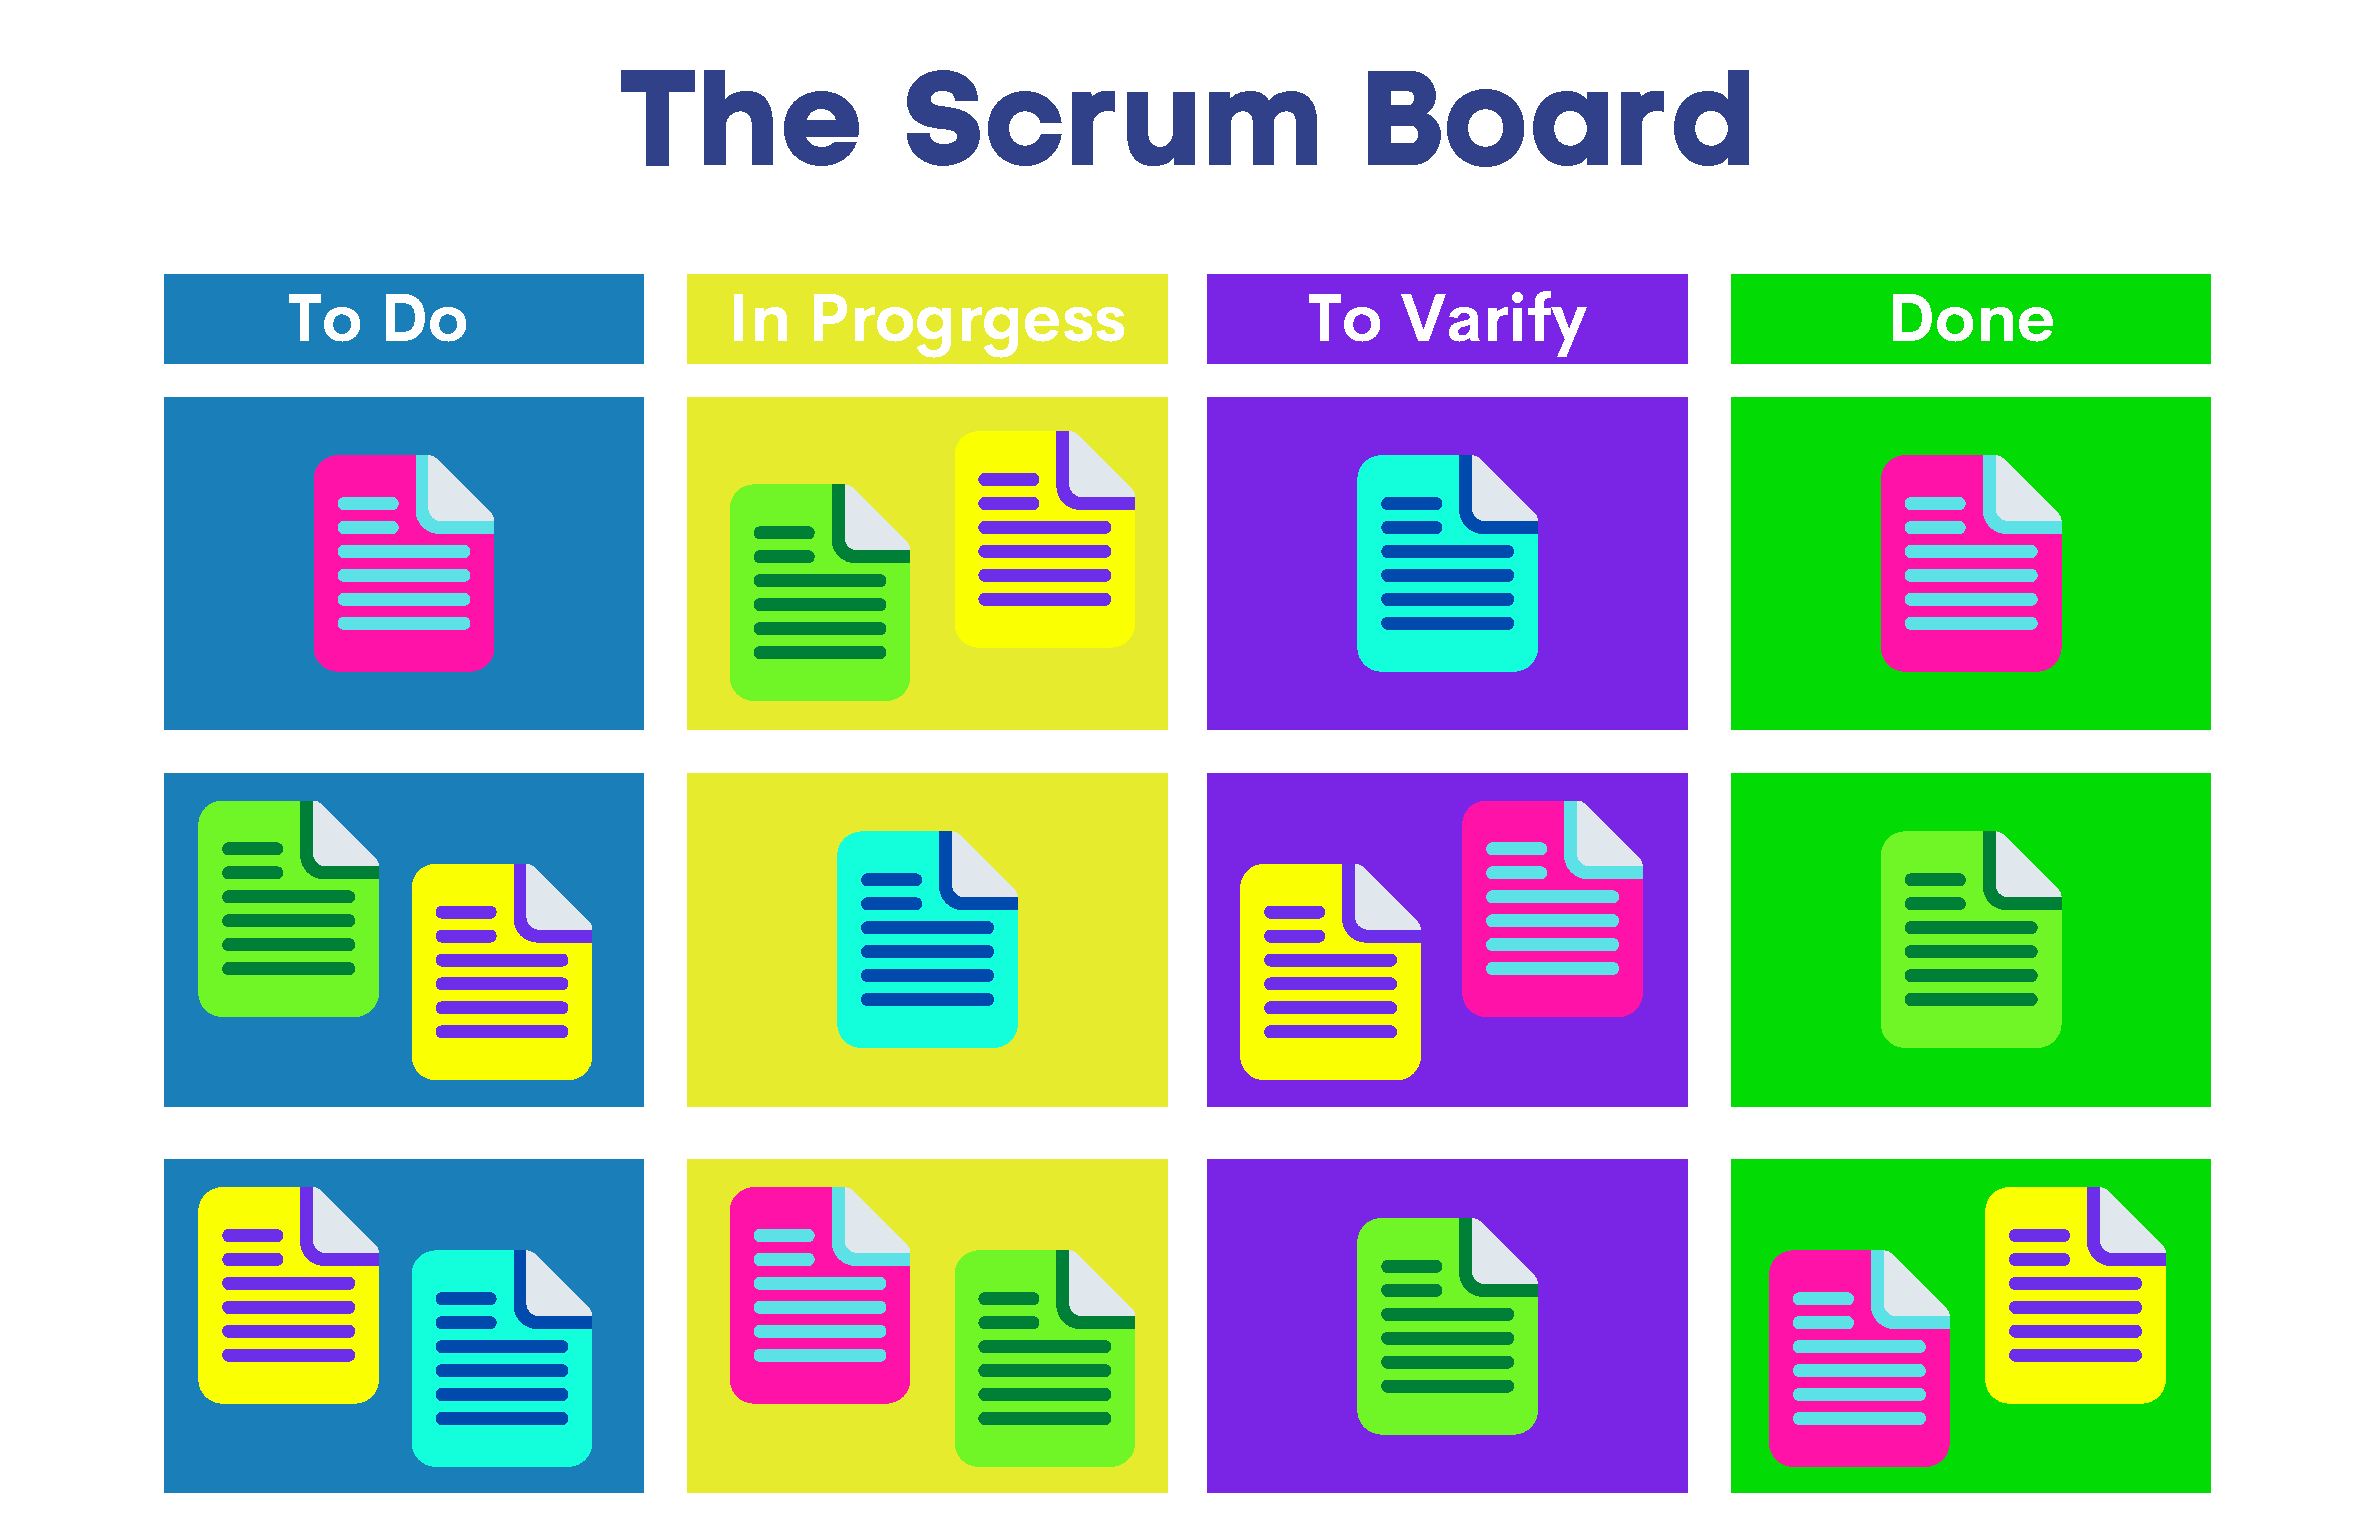
\includegraphics[width=1\textwidth]{images/scrum_board}
    \caption{Project Management Agile Scrum Board Template}
    \label{fig:scrum_board}
\end{figure}

\item \textbf{Testing and Product Demonstration}\\

Our system's stack holders have been reviewed, and thus this phase is mainly the modification phase depending on the results of the study. The activities done were to be turned into a workable product that would be subjected to full life cycle testing. Every sprint that was done was displayed to the stack holders, who included students, teachers, and other relevant authorities, in order to get their approval and opinion on the overall solution. We got positive feedback from the stack holders, and in the majority of instances, they stated their satisfaction with the solution that we provided. In response to our request for recommendations, a portion of them provided us with some suggestions for improvements to numerous aspects of the application. We definitely implemented a significant number of them and integrated them into the final system.

\item \textbf{Retrospective and the next sprint planning}\\

After this phase was completed, it was necessary to examine what had gone well and what might be improved for the following level. We also spoke about the lessons gained and the hazards of any specific challenges or problems that came up throughout the course of the project. We discussed our next sprint, which will consist of future development. We want to include additional features into the system over time, and eventually transform it into a dependable and fully working university administration system. Our team is sure that they will be able to do this with the present information and more research. As a consequence, there will be no need for paper in administration. All of the formal duties will take less time than they have in the past. In the interim, we will undoubtedly maintain the system in order to ensure that it continues to function as an uninterrupted service provider application.


\end{enumerate}

Each and every member of our team has made an equal contribution to the project, from the beginning of the planning phase to the completion of the system's final implementation. We attempted to create a better system than the present one, and after hundreds of proposals were discussed and rejected by all of us, we were eventually successful. In order to accomplish this project, we attempted to make the best possible use of existing technology. During the course of the project, we discovered a great deal of new information while being stuck on challenges we had never encountered before. Projects might be conducted carelessly if adequate project management principles are not followed, putting them at a much greater risk of failure, delay, and going over budget. Knowing the foundations of project management increased our chances of effectively completing a project.
According to this procedure we complete all of the steps of SDLC and our project completes.
\footnotetext[1]{Scrum is an agile development methodology used in the development of Software based on an iterative and incremental processes. Scrum is adaptable, fast, flexible and effective agile framework that is designed to deliver value to the customer throughout the development of the project.}

\footnotetext[2]{Trello is a web-based, Kanban-style, list-making application and is developed by Trello Enterprise, a subsidiary of Atlassian. It is a visual collaboration tool that enables one to organize and prioritize projects in a fun, flexible, and rewarding way. A Trello board is a series of lists, with a bunch of cards attached and packed full with powerful features and automation. [website: www.trello.com]}

\footnotetext[3]{Google Meet is a video-communication service developed by Google. It is one of two apps that constitute the replacement for Google Hangouts, the other being Google Chat. website[www.meet.google.com]}

\footnotetext[4]{GitHub is a provider of Internet hosting for software development and version control using Git. It offers the distributed version control and source code management functionality of Git, plus its own features. It lets us and others work together on projects from anywhere. [website: www.github.com]}

\clearpage